\documentclass{article}
\usepackage[utf8]{inputenc}

\usepackage[utf8]{inputenc}
% to set spacing of page margins
\usepackage[margin=2cm,nohead]{geometry}
% to include images
\usepackage{graphicx}
% to automatically create paragraphs when doing so in the code
\usepackage{parskip}

% to not indent new paragraphs
\setlength{\parindent}{0pt}

% line spacing
\usepackage{setspace}
\doublespacing
%\onehalfspacing

\begin{document}

\section*{IT19tb WIN7 S5 Aufgabe 1}
Leo Rudin \& Stefan Teodoropol

Gleichung umgeschrieben als Funktion: \(f(x) = e^{x^2} + x^{-3} - 10\)\\
Ableitung: \(f'(x) = 2xe^{x^2} - 3x^{-4}\)

\begin{figure}[h!]
\centering
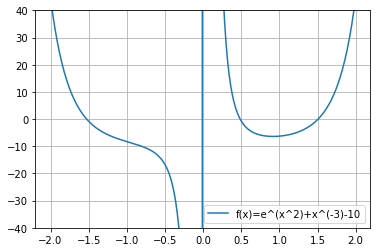
\includegraphics[scale=0.7]{plot_aufg1.png}
\caption{Plot der Funktion; Nullstellen scheinen ungefähr bei -1.5, 0.5 und 1.5 zu sein.}
\label{fig:plot_aufg1b.png}
\end{figure}

\subsubsection*{Newton-Verfahren:}

\(x_{n+1} = x_n - \frac{f(x_n)}{f'(x_n)}\)\\
Startwert \(x_0 = 2\)

\(x_1 = 2 - \frac{e^{2^2} + 2^{-3} - 10}{2*2*e^{2^2} - 3*2^-4} = 1.7950\)\\
\(x_2 = 1.7950 - \frac{e^{1.7950^2} + 1.7950^{-3} - 10}{2*1.7950*e^{1.7950^2} - 3*1.7950^-4} = 1.6251\)\\
\(x_3 = 1.6251 - \frac{e^{1.6251^2} + 1.6251^{-3} - 10}{2*1.6251*e^{1.6251^2} - 3*1.6251^-4} = 1.5308\)\\
\(x_4 = 1.5308 - \frac{e^{1.5308^2} + 1.5308^{-3} - 10}{2*1.5308*e^{1.5308^2} - 3*1.5308^-4} = 1.5308\)

Der Startwert \(x_0 = 2\) konvergiert gegen 1.5308. Die Nullstelle scheint im Interval [1.5308,1.5309] zu liegen.

\newpage
\subsubsection*{Einfaches Newton-Verfahren:}

\(x_{n+1} = x_n - \frac{f(x_n)}{f'(x_0)}\)\\
Startwert \(x_0 = 0.5\)\\
\(f'(0.5) = -46.716\)

\(x_1 = 0.5 - \frac{e^{0.5^2} + 0.5^{-3} - 10}{-46.716} =0.4847\)\\
\(x_2 = 0.4847 - \frac{e^{0.4847^2} + 0.4847^{-3} - 10}{-46.716} =0.4857\)\\
\(x_3 = 0.4857 - \frac{e^{0.4857^2} + 0.4857^{-3} - 10}{-46.716} =0.4856\)\\
\(x_4 = 0.4856 - \frac{e^{0.4856^2} + 0.4856^{-3} - 10}{-46.716} =0.4856\)

Der Startwert \(x_0 = 0.5\) konvergiert gegen 0.4856. Die Nullstelle scheint im Interval [0.4856,0.4857] zu liegen.

\subsubsection*{Sekantenverfahren:}
\(x_{n+1} = x_n - \frac{x_n - x_{n-1}}{f(x_n) - f(x_{n-1})} * f(x_n)\)\\
Startwerte \(x_0 = -1.0, x_1 = -1.2\)

\(x_2=-1.2-\frac{-1.2-(-1.0)}{(e^{-1.2^2}+(-1.2^{-3})- 10)-(e^{-1.0^2}+(-1.0^{-3})-10)}*(e^{-1.2^2}+(-1.2^{-3})-10)=-1.8610\)\\
\(x_3=-1.8610-\frac{-1.8610-(-1.2)}{(e^{-1.8610^2}+(-1.8610^{-3})- 10)-(e^{-1.2^2}+(-1.2^{-3})-10)}*(e^{-1.8610^2}+(-1.8610^{-3})-10)=-1.3494\)\\
\(x_4=-1.3494-\frac{-1.3494-(-1.8610)}{(e^{-1.3494^2}+(-1.3494^{-3})- 10)-(e^{-1.8610^2}+(-1.8610^{-3})-10)}*(e^{-1.3494^2}+(-1.3494^{-3})-10)=-1.4326\)\\
\(x_5=-1.4326-\frac{-1.4326-(-1.3494)}{(e^{-1.4326^2}+(-1.4326^{-3})- 10)-(e^{-1.3494^2}+(-1.3494^{-3})-10)}*(e^{-1.4326^2}+(-1.4326^{-3})-10)=-1.5594\)

Die Nullstelle scheint im Interval [-1.4326,-1.5594] zu liegen.

\end{document}
